\newcommand{\institut}{Institut f\"ur Hochfrequenzund
Halbleiter-Systemtechnologien}
\newcommand{\fachgebiet}{Halbleiterbauelemente}
\newcommand{\veranstaltung}{Praktikum Technologie und Bauelemente der
Halbleitertechnik}
\newcommand{\pdfautor}{Alona Siebert (303843), Özgü Dogan (326048), Dirk Babendererde (321 836), Thomas Kapa (325 219)}
\newcommand{\autor}{Alona Siebert (303843)\\ \"Ozg\"u Dogan (326048)\\ Dirk Babendererde (321 836)\\ Thomas Kapa (325 219)}
\newcommand{\gruppe}{Gruppe:1}
\newcommand{\betreuer}{Betreuer: Clemens Helfmeier, Philipp Scholz}


\newcommand{\pdftitle}{Technologie und Bauelemente der
Halbleitertechnik}
\newcommand{\prototitle}{Protokollvorlage}

\input{../../packages/tu_header_9}

\setcaptionwidth{7.5cm}

\begin{document}


%     \lstinputlisting{./praktikum6.sce}



%---------------------------------------------------------------------
%---------------------------------------------------------------------
%---------------------------------------------------------------------

\section{Kennlinie}
\begin{quote}

\end{quote} %sec Kennlinie

%--------------------------------------------------------------------
%--------------------------------------------------------------------

\section{Schaltverhalten}
\begin{quote}

In diesem Versuch soll Schaltverhalten bei Strom- und Spannungssprüngen untersucht werden.
Ein Maß für die Geschwindigkeit mit der die Diode schalten kann ist die Minoritätsträgerlebensdauer.
Der Schaltvorgang hält an, bis diese auf- bzw. abgebaut sind. Daher ist es Ziel dieses Versuches über
zwei unterschiedliche Verfahren diese Ladungsträgerlebensdauer zu bestimmen. Dies ist zum einen der
Stromausschaltvorgang und zum anderen die Stromkommutierung.\\

Zunächst sollen das ideale und das reale Schaltverhalten gegenüber gestellt werden. Das ideale Verhalten
charakterisiert sich durch verzögerungs- und verlustfreies Schalten. Die zu messenden Dioden zeigen allerdings 
durch Energiespeicher wie die Sperrschicht- und die Diffusionskapazität kein ideales Schaltverhalten. \\

Dabei ist die Charakteristik des Schaltverhaltens davon abhängig, ob es sich um ein Spannungs- oder Stromsprung 
und einen Ein- oder Ausschaltvorgang handelt. Um das Verständnis für diese Vorgänge zu verbessern, soll im Folgenden 
näher auf einige Beispiele eingegangen werden.\\

Bei einem Einschaltstromsprung werden zwei Fälle unterschieden: Die starke und die schwache Injektion. Ob starke oder 
schwache Injektion vorliegt richtet sich nach der Ladungsträgeranzahl, die von der einen Seite des pn-Überganges als 
Majoritätsträger auf die andere Seite als Minoritätsträger gelangen. Ist die Anzahl der auf der anderen Seite 
ankommenden nun Minoritäten in etwa so groß, oder größer wie die Majoritäten spricht man von starker Injekion.
Andernfalls spricht man von schwacher Injektion.\\
Wie in Bild \ref{fig:Stromeinschalten} zu erkennen, spielt in den beiden Fällen der Bahnwiderstand eine
unterschiedliche Rolle. Nach Shockley ist der Bahnspannungsabfall für schwache Injektion zu vernachlässigen. 
Mit Hilfe der Boltzmanfaktoren lässt sich ein logarthmischer Verlauf der Spannung über der RLZ herleiten. 
Dieser ist in der Abbildung \ref{fig:Stromeinschalten} in der grob gestrichelten Kennlinie zu erkennen. 
Man könnte vermuten, dass ohne den Bahnwiderstand nur der kapazitive Anteil zur Wirkung kommt und die Spannung 
daher kaum springen darf.\\
Kommt hingegen der Einfluss des Bahnwiderstandes bei der starken Injektion hinzu, dann kann ein heftiger 
Spannungssprung erfolgen. Der zusammengefasste Spannungsverlauf ist in Bild \ref{fig:Stromeinschalten} an der 
durchgezogenen Kennlinie zu erkennen. Durch den Bahnwiderstand bekommt die Diode vergleichbar mit Zuleitungen
einen induktiven Charakter und die Spannung kann springen.

    \begin{figure}[h]
        \centering
        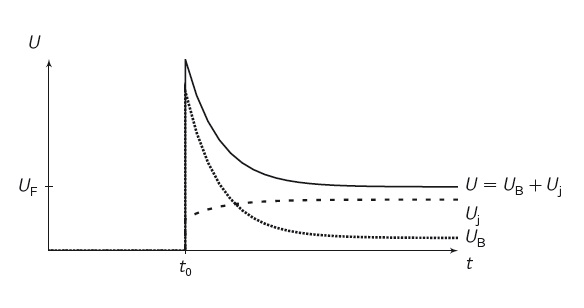
\includegraphics[scale=1]{Bilder/Stromeinschalten}
        \caption{Spannungsverlauf beim Stromeinschaltsprung für starke und schwache Injektion \footnotemark} 
        \label{fig:Stromeinschalten}
    \end{figure} 
         \footnotetext{Prof. Boit, Clemens Helfmeier, Philipp Scholz: Laborskript Technologie und Bauelemente der
Halbleitertechnik (SS 2012), S. 78}
   
   \newpage   

      \begin{table}[h]
               \begin{addmargin}[-1cm]{3cm}
               \centering
                    \begin{tabular}{|p{5cm}|p{11.2cm}|}
         \hline
         Messung  &   Werte\\
         \hline
         Ausschaltvorgang  & $I_{F}=10, 50, 100, 150 mA$\\
   
         \hline
         Stromkommutierung  &  $I_{R0}=15,30,60,90,120 mA$\\ 
         
         \hline
         

                    \end{tabular}
                \end{addmargin}
             \caption{Messarten}
          \label{Messarten}
      \end{table} 
     
      \vspace{2em}

      \begin{table}[h]
    	        \begin{addmargin}[-1cm]{3cm}
    	          \centering
                     \begin{tabular}{|p{3cm}|p{3cm}|p{10.2cm}|}
         \hline
         Messung                 & Die/Diode/Wafer & gemessen\\ 
         \hline
         $R_{B} für I_{F}=10 mA$ &           &                  \\
                                 &           &                  \\ 
                                 &           &                  \\
                                 &           &                  \\ 
                                 &           &                  \\
                                 &           &                  \\ 
                                 &           &                  \\
                                 &           &                  \\ 
                                 &           &                  \\
                                 &           &                  \\ 
                                 &           &                  \\
                                 &           &                  \\ 
                                 &           &                  \\
         \hline
         $R_{B} für I_{F}=50 mA$ &           &                  \\
                                 &           &                  \\ 
                                 &           &                  \\
                                 &           &                  \\ 
                                 &           &                  \\
                                 &           &                  \\ 
                                 &           &                  \\
                                 &           &                  \\ 
                                 &           &                  \\
                                 &           &                  \\ 
                                 &           &                  \\
                                 &           &                  \\ 
                                 &           &                  \\
         \hline
         $R_{B} für I_{F}=100 mA$ &          &                  \\
                                 &           &                  \\ 
                                 &           &                  \\
                                 &           &                  \\ 
                                 &           &                  \\
                                 &           &                  \\ 
                                 &           &                  \\
                                 &           &                  \\ 
                                 &           &                  \\
                                 &           &                  \\ 
                                 &           &                  \\
                                 &           &                  \\ 
                                 &           &                  \\
         \hline
         $R_{B} für I_{F}=150 mA$ &          &\\
                                 &           &                  \\ 
                                 &           &                  \\
                                 &           &                  \\ 
                                 &           &                  \\
                                 &           &                  \\ 
                                 &           &                  \\
                                 &           &                  \\ 
                                 &           &                  \\
                                 &           &                  \\ 
                                 &           &                  \\
                                 &           &                  \\ 
                                 &           &                  \\
   
         \hline

                     \end{tabular}
                 \end{addmargin}
             \caption{Messwerte}
           \label{Messwerte1}
        \end{table}
      
       \vspace{2em}
       
       \begin{table}[h]
    	   \begin{addmargin}[-1cm]{3cm}
    	         \centering
                      \begin{tabular}{|p{3cm}|p{3cm}|p{10.2cm}|}
         \hline
         Messung                 & Die/Diode/Wafer & gemessen\\ 
         \hline
         $\tau für I_{F}=150 mA$ &        & \\
                                 &           &                  \\ 
                                 &           &                  \\
                                 &           &                  \\ 
                                 &           &                  \\
                                 &           &                  \\ 
                                 &           &                  \\
                                 &           &                  \\ 
                                 &           &                  \\
                                 &           &                  \\ 
                                 &           &                  \\
                                 &           &                  \\ 
                                 &           &                  \\
         \hline
         $t_{s}$                 &           & \\ 
                                 &           &                  \\ 
                                 &           &                  \\
                                 &           &                  \\ 
                                 &           &                  \\
                                 &           &                  \\ 
                                 &           &                  \\
                                 &           &                  \\ 
                                 &           &                  \\
                                 &           &                  \\ 
                                 &           &                  \\
                                 &           &                  \\ 
                                 &           &                  \\
         \hline
         $Q_{s}$                 &           &\\
                                 &           &                  \\ 
                                 &           &                  \\
                                 &           &                  \\ 
                                 &           &                  \\
                                 &           &                  \\ 
                                 &           &                  \\
                                 &           &                  \\ 
                                 &           &                  \\
                                 &           &                  \\ 
                                 &           &                  \\
                                 &           &                  \\ 
                                 &           &                  \\
         \hline
         $\tau$                  &           &\\
                                 &           &                  \\ 
                                 &           &                  \\
                                 &           &                  \\ 
                                 &           &                  \\
                                 &           &                  \\ 
                                 &           &                  \\
                                 &           &                  \\ 
                                 &           &                  \\
                                 &           &                  \\ 
                                 &           &                  \\
                                 &           &                  \\ 
                                 &           &                  \\
         \hline

                           \end{tabular}
                    \end{addmargin}
             \caption{Messwerte}
         \label{Messwerte2}
      \end{table}
      
      \vspace{2em}
      
      \begin{table}[h]
                 \begin{addmargin}[-1cm]{3cm}
    	         \centering
                     \begin{tabular}{|p{3cm}|p{3cm}|p{10.2cm}|}
         \hline
         Messung                 & Die/Diode/Wafer & gemessen\\ 
         \hline
         Tempertatur  &    & \\
                                 &           &                  \\ 
                                 &           &                  \\
                                 &           &                  \\ 
                                 &           &                  \\
                                 &           &                  \\ 
                                 &           &                  \\
                                 &           &                  \\ 
                                 &           &                  \\
                                 &           &                  \\ 
                                 &           &                  \\
                                 &           &                  \\ 
                                 &           &                  \\
         \hline
         Vorwärtsstrom  &    & \\ 
                                 &           &                  \\ 
                                 &           &                  \\
                                 &           &                  \\ 
                                 &           &                  \\
                                 &           &                  \\ 
                                 &           &                  \\
                                 &           &                  \\ 
                                 &           &                  \\
                                 &           &                  \\ 
                                 &           &                  \\
                                 &           &                  \\ 
                                 &           &                  \\
         \hline
         Rückwärtsstrom  &     &\\
                                 &           &                  \\ 
                                 &           &                  \\
                                 &           &                  \\ 
                                 &           &                  \\
                                 &           &                  \\ 
                                 &           &                  \\
                                 &           &                  \\ 
                                 &           &                  \\
                                 &           &                  \\ 
                                 &           &                  \\
                                 &           &                  \\ 
                                 &           &                  \\
         \hline
                     \end{tabular}
                  \end{addmargin}
             \caption{Sonstige Angaben zur Messung}
         \label{AngabenZurMessung}
      \end{table} 
      
      \noindent
      
       \vspace{2em}
      
\end{quote} %sec Schaltverhalten

%--------------------------------------------------------------------
%--------------------------------------------------------------------

\section{Emissionsmessung}
\begin{quote}

\end{quote} %sec Emissionsmessung

%--------------------------------------------------------------------
%--------------------------------------------------------------------
\newpage

\begin{thebibliography}{999}

% \bibitem{Boris}Boris Henckell: Ein Paar sachen geklaut.. ähhh inspirationen geholt
% \href{http://www.krachler.com/fileadmin/user_upload/arbeiten/Reglersynthese_Christian_Krachler.pdf}{Reglersynthese nach dem Frequenzkennlinienverfahren}, S16, S22, 08.05.2012


% Name, Vorname.; evtl. Name2, Vorname2.: Titel des Dokumentes
% oder Buches, Zeitschrift/Verlag/URL (Auflage, Erscheinungsort, -jahr), ggf. Seitenzahlen
%\bibitem [Wiki10] {DigitaleMesskette2} \url{www.wikipedia.org}, Zugriff 22.03.2010

\bibitem [1]{TBH} Prof. Boit, Clemens Helfmeier, Philipp Scholz: Laborskript Technologie und Bauelemente der
Halbleitertechnik (SS 2012)
\end{thebibliography}

\end{document}
